  \subsection{Ejercicio 7}

  Para estudiar la performance del Round-Robin variando los cuantos creamos el lote7 y realizamos varias simulaciones. Variamos los quantums entre 1 y 10 inclusive y evaluamos el throughput y INSERTAR SEGUNDA M\'ETRICA con 2 y 4 n\'ucleos. Como las tareas TaskConsola son pseudoaleatorias,
  para cada seleccio\'on de par\'ametros corrimos 10 simulaciones y graficamos el promedio con la variaci\'on estandard.

  \begin{figure}
  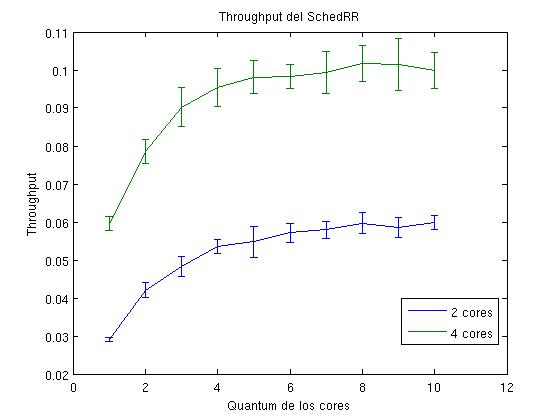
\includegraphics[scale=0.6]{images/TH.jpg}
  \caption{Throughput para SchedRR con dos y cuatro n\'ucleos}
  \end{figure}

  En la figura 6 se muestran los resultados del throughput. En la misma se observa que (considerando las desviaciones) el throughput aumenta al aumentar el quantum, tanto para 2 como 4 n\'ucleos. Esto tiene mucho sentido, ya que se
  gasta menos tiempo en cambios de contexto y es menos probable que un proceso cambie de CPU, bajando el costo total de migraci\'on de procesos entre CPUs. Obviamente, este crecimiento converge, ya que el tiempo que tardan en terminar los procesos est\'a acotado por
  el uso total del CPU dividido la cantidad de n\'ucleos, por lo que el throughput tambi\'en converge.
